\documentclass[11pt, a4paper, twocolumn]{article}
\usepackage[utf8]{inputenc}
\usepackage{url}
\usepackage{hyperref}
\usepackage[margin=1.5cm]{geometry}
\usepackage{graphicx}
\usepackage{amsmath}
\usepackage{amssymb}


\title{
\begin{flushleft}

\includegraphics[width=3.5cm]{images/uibknew.eps}
\hfill

\includegraphics[width=1.8cm]{images/igslogo.png}
\hspace{0.3cm}

\includegraphics[width=0.9cm]{images/iislogo.png}
\end{flushleft}\vspace{0.5cm}
Visual Computing Project Report}
\author{Susanne Musterfrau \& Max Mustermann}

%-- more dense bibstyle
\let\oldthebibliography\thebibliography
\let\endoldthebibliography\endthebibliography
\renewenvironment{thebibliography}[1]{
  \begin{oldthebibliography}{#1}
    \setlength{\itemsep}{0em}
    \setlength{\parskip}{0em}
}
{
  \end{oldthebibliography}
}

\begin{document}


\maketitle

\thispagestyle{empty}


\section*{Introduction}
Shortly describe the task of the project.
Motivate and give the problem statement of the task.
Add at least one reference (book \cite{Bridson08}, paper \cite{Zuenko20}, homepage \cite{lighthouse_timer}) via the 'sources.bib' and the 'cite' command.
One final short paragraph about the own solution and the final results.

\section*{Background}
Shortly describe the necessary theory, e.g.~Blinn-Phong illumination model, fourier transformation, Gaussian blur.
Show the employed theoretical formulas and/or more specialized math.
\begin{align}
    I_S = k_S M_S I_L \left( \cos \frac{\phi}{2} \right)^m = k_S M_S I_L \left( \mathbf{n} \cdot \mathbf{h} \right)^m
\end{align}

\section*{Method}
Describe the method(s), or most essential part(s) of the method you used to solve the task.
Also, some \textbf{short} implementation notes can be added here. Cite your sources accordingly.
%
\begin{figure}[!b]
 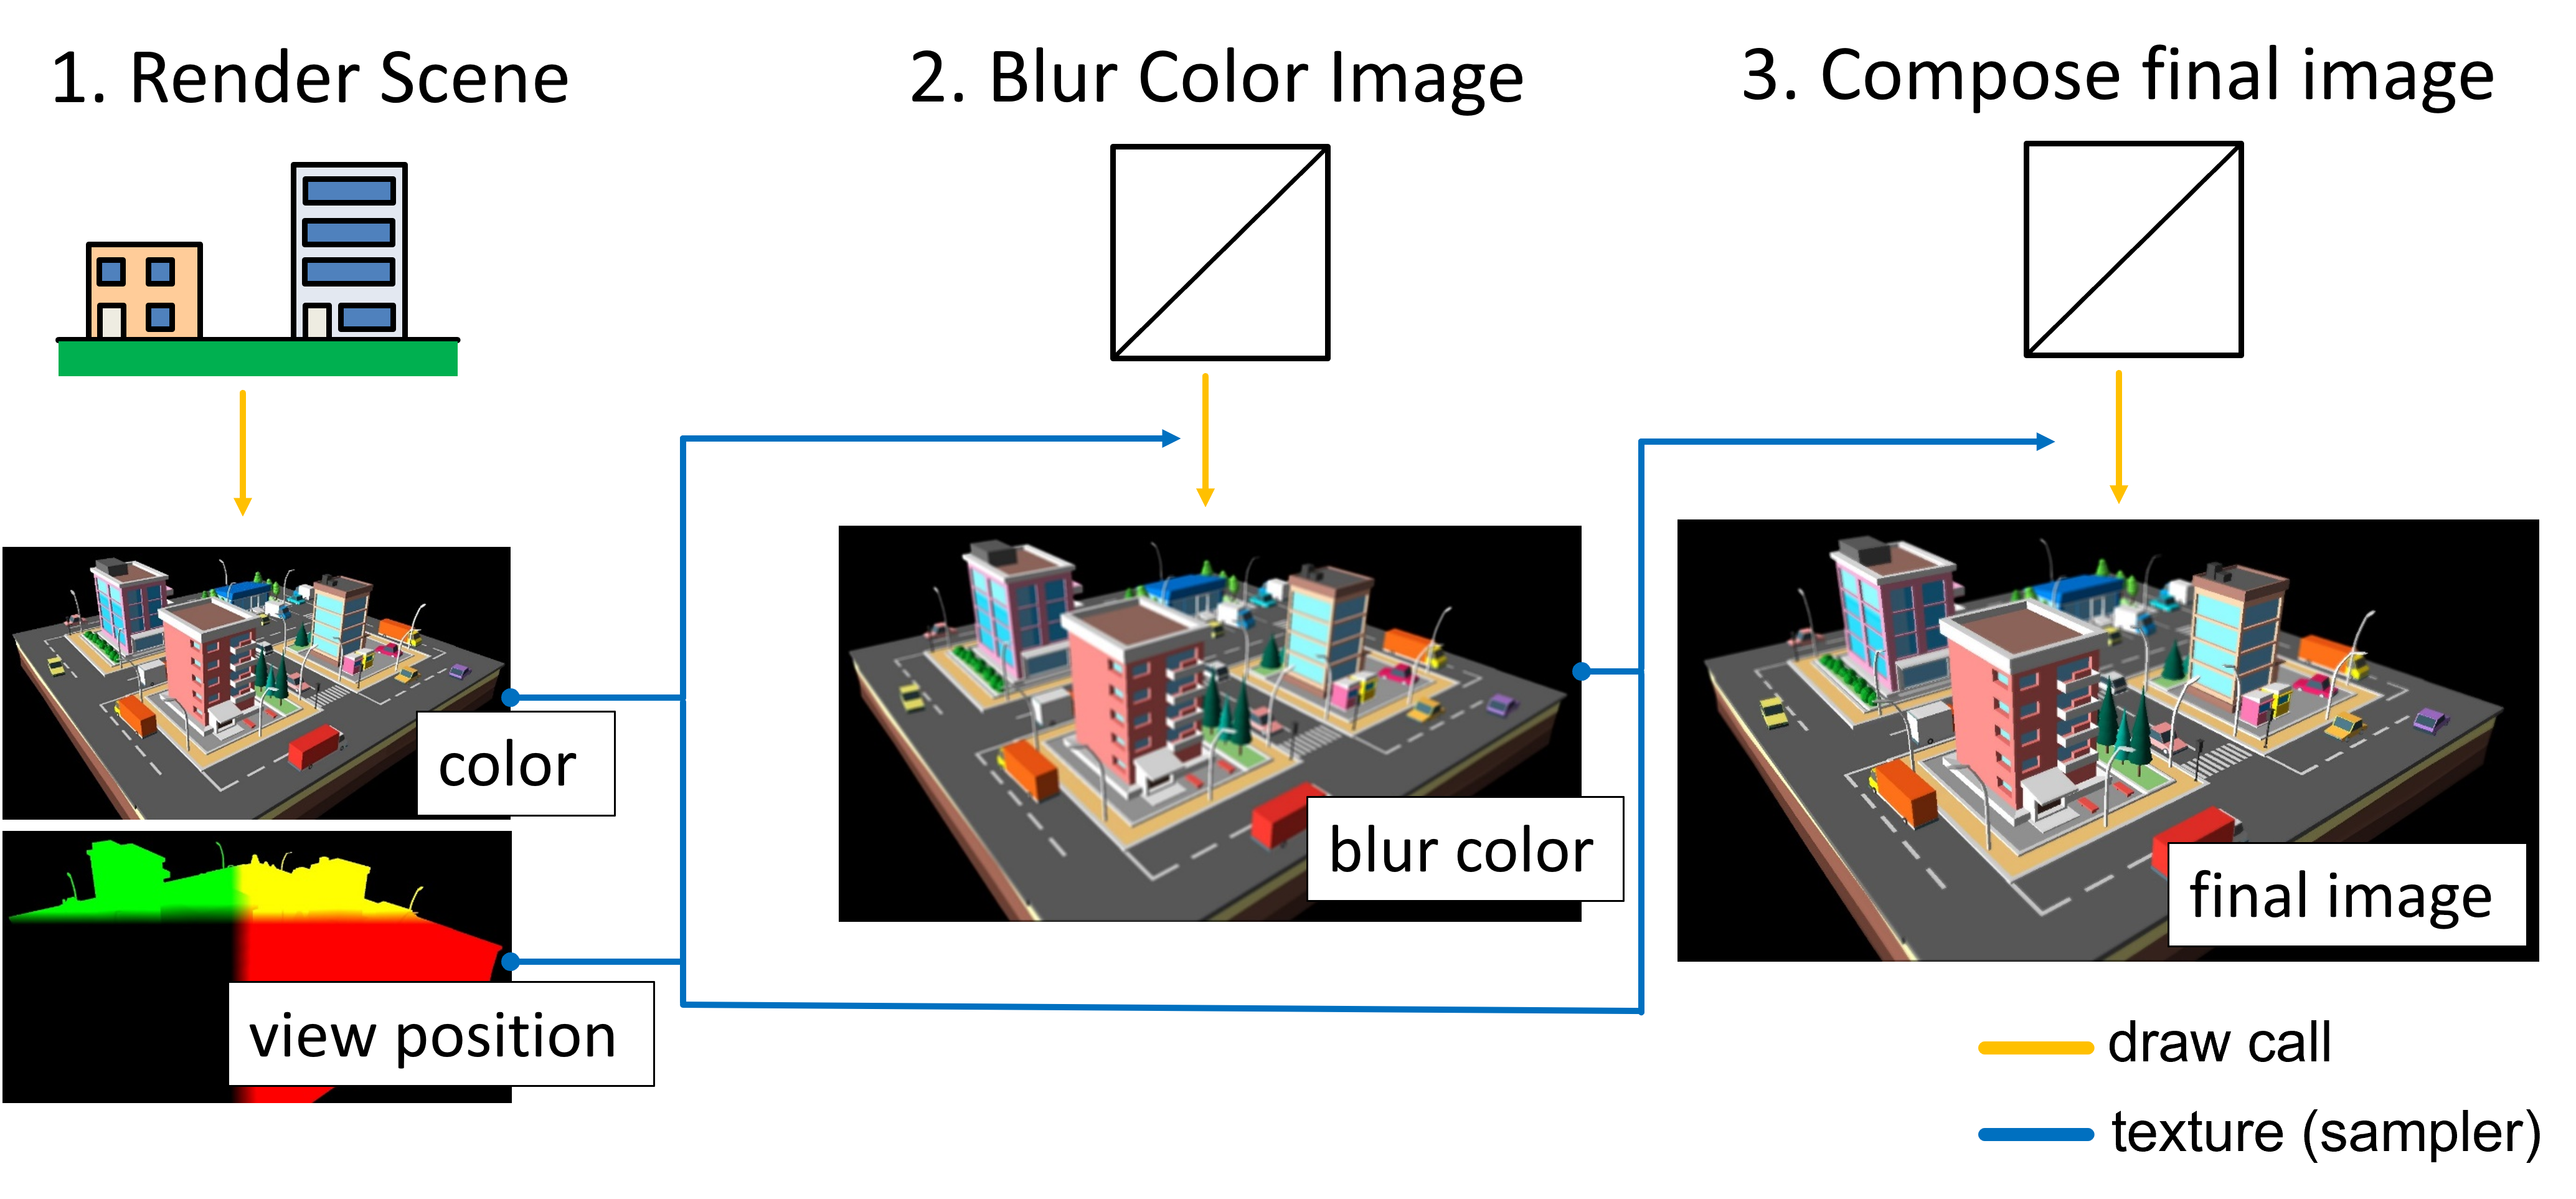
\includegraphics[width=1.0\columnwidth]{images/blur_pipeline.png}
 \centering
 \caption{Abstract render pass pipeline for \emph{post-process depth-of-field}}
 \label{fig:blur_pipeline}
\end{figure}

\section*{Results}
Describe the experiments/scene.
If there are visual results show some images; make sure they are of importance.
If there are measurements possible for demonstration add plots; e.g.~accuracy of classification or GPU runtime for each frame with \texttt{OpenGL Timer Query} \cite{lighthouse_timer}.
%
\begin{figure}[h]
    \centering
    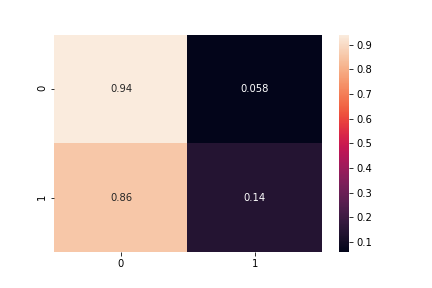
\includegraphics[width=0.4\textwidth]{images/confusion_matrix.png}
    \caption{Normalized Confusion Matrix}
    \label{fig:conf_matrix}
\end{figure}

\section*{Conclusion}
Summarize what was done.
Also add some of your findings, challenges, and problems you encountered. 
What are the limits?
What could be improved?\\
~\\
\textbf{More remarks:}
Do not modify the layout (font, margins, etc.).
Avoid subsections and prefer a bold paragraph start.
Try to write complete but \mbox{succinct}.
Follow the section layout: introduction, background, method, results, and conclusion.
But, feel free to adjust if it makes sense. \\
~\\
\textbf{Amount:} The report must have 4 \textbf{filled} pages (\textbf{without references}); Use a reasonable amount and size for images and plots.

\bibliographystyle{plain}
\bibliography{sources}{}

%\bibliographystyle{ieeetr}



\end{document}
